\section{Grundlagen} 
In diesem Abschnitt werden die Grundlagen für die Thesis erläutert. 

\subsection{Adversarial Attacks}
Adversarial Attacks sind ein Phänomen im Bereich des Deep Learning, das in den letzten Jahren zunehmend an Bedeutung gewonnen hat. Szegedy et al. \cite{szegedy_intriguing_2014} haben erstmals festgestellt, dass es möglich ist, die Vorhersage eines neuronalen Netzwerks beliebig zu verändern, wenn eine nicht wahrnehmbare, nicht zufällige Störung, sogenannte ``adversarial examples'', auf ein Testbild angewendet wird. Diese Störungen werden durch Optimierung der Eingabe gefunden, indem der Vorhersagefehler maximiert wird. In dieser Thesis werden für diese Art von Angriffen der heute gebräuchlichere Begriff ``Adversarial Attacks'' verwendet.

\subsubsection{Schema eines Adversarial Attack} 
Die Abbildung \ref{fig:grundlagen} illustriert den allgemeinen Adversarial Attack auf ein beliebiges Model $c$. 

\begin{figure}[H]
    \centering
    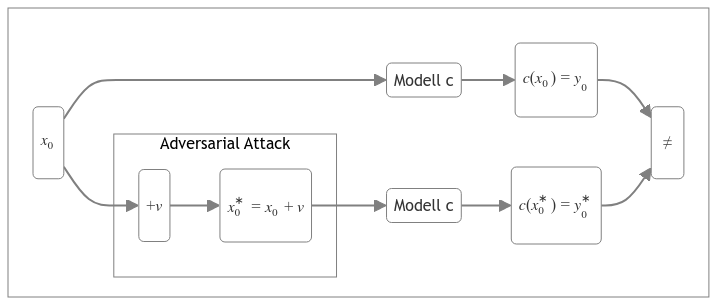
\includegraphics[width=0.8\linewidth]{01-images/02-grundlagen/adversarial-attack.png}
    \caption{Vorgang einer Attacke}
    \label{fig:grundlagen}
\end{figure}

\begin{align*}
    x_0,      &\text{ der Eingabewert, dies kann ein Signal, Bild oder ein sonstiges Format sein.} \\
    v,        &\text{ der Adversarial Attack.} \\
    x_0^{*},  &\text{ der veränderte, attackierte Eingabewert.} \\
    c,        &\text{ das Modell, welches die Eingabe verarbeitet und Output generiert.} \\
    y_0,      &\text{ der Output des Modells durch den unveränderten Eingabewert.} \\
    y_0^{*},  &\text{ der Output des Modells durch den attackierte Eingabewert.} \\
    \neq,     &\text{ der Output von $y_0$ und $y_0^{*}$ ist nicht gleich.} \\
\end{align*} 

\newpage

\subsubsection{Beispiele für Adversarial Attacks} 
Ein Beispiel eines physischen Adversarial Attacks ist das ``Adversarial T-Shirt'' von Xu et al. \cite{xu_adversarial_2020}. Dieses T-Shirt ist mit speziellen Mustern bedruckt, die darauf ausgelegt sind, Objekterkennungssysteme zu täuschen. 

Ein weiteres Beispiel, der ``One Pixel Attack'' von Su et al. \cite{su_one_2019} zielt darauf ab, Deep Neural Networks durch die Modifikation eines einzigen Pixels in einem Bild zu täuschen. Diese Methode offenbart die hohe Sensitivität von \acrlong{dnn}s gegenüber minimalen Veränderungen in den Eingabedaten. Dabei wird das effektivste Pixel sowie dessen Farbänderung ermittelt, um eine Fehlklassifizierung durch das Netzwerk zu erzeugen. 

\subsection{Universal Adversarial Attacks auf Bildklassifikation} \label{chap:Universal Adversarial Attacks auf Bildklassifikation}
Die Hauptstudie, ``Universal Adversarial Perturbation'' von Moosavi-Dezfooli et al. \cite{moosavi-dezfooli_universal_2017}, bildet die Grundlage für den Perturbationsalgorithmus dieser Bachelorthesis. Die Autoren demonstrieren die Existenz von universellen Perturbationen, die mit hoher Erfolgsrate fehlerhafte Klassifizierungen über verschiedene Bilder hinweg induzieren können. Diese Perturbationen führen unabhängig vom Bildinhalt zu einer Fehlklassifikation des Modells. Diese Methode gehört zu den White-Box-Attacken, bei denen die Gewichte des anzugreifenden Modells bekannt sein müssen, um einen erfolgreichen Angriff durchführen zu können.

\subsubsection{Bisherige Herausforderungen bei der Verteidigung}
Im Paper von Moosavi-Dezfooli et al. \cite{moosavi-dezfooli_universal_2017} wird die Effektivität von Fine-Tuning-Techniken zur Verbesserung der Robustheit von \acrlong{dnn}s gegenüber \acrlong{uap}s untersucht. Dazu wurde die VGG-F-Architektur verwendet und dem Trainingssatz mit einer Wahrscheinlichkeit von 50\% universelle Perturbationen addiert, die zufällig aus einem Pool von 10 verschiedenen \acrshort{uap}s ausgewählt wurden.

Das Fine-Tuning zeigte eine gewisse Verbesserung der Netzwerkrobustheit. Jedoch blieb das Netzwerk trotz der Anpassungen weiterhin anfällig für \acrshort{uap}s. Mehrfaches Fine-Tuning führte nicht zu einer signifikanten weiteren Verbesserung.

\newpage

\subsection{Anwendungsfall} 
Angesichts der Vielfalt an möglichen Konfigurationen für die Generierung der Attacken und der \Gls{robustifizierung} der Modelle basieren unsere Entscheidungen bezüglich der Parameterwahl auf einem speziell ausgewählten Anwendungsfall. 

Im Gegensatz zum Paper von Moosavi-Dezfooli et al. \cite{moosavi-dezfooli_universal_2017} liegt der Schwerpunkt dieser Arbeit auf der Anwendung von \acrlong{uap}s auf binäre medizinische Klassifikationsmodelle, sowie deren \Gls{robustifizierung}. Der Algorithmus wird so modifiziert, dass er gezielt 20\% der tatsächlich positiven Bilder fälschlicherweise als negativ klassifiziert, was dazu führen könnte, dass bei einem von fünf Patienten mit einem positiven Befund dieser übersehen wird und folglich kritische Krankheitszustände nicht erkannt und nicht angemessen behandelt werden.

Die Herausforderung bei der Generierung der Perturbationen besteht darin, diese so zu gestalten, dass sie minimal und für das menschliche Auge schwer erkennbar sind. Eine offensichtliche Änderung des Bildes im medizinischen Kontext kann sofort Misstrauen erwecken und somit schnell identifiziert werden. Durch den subtilen Einsatz von Perturbationen soll die Balance zwischen der Wirksamkeit der Angriffe und ihrer Unauffälligkeit optimiert werden. 

Zusätzlich zum Paper von Moosavi-Dezfooli et al. \cite{moosavi-dezfooli_universal_2017} werden in dieser Arbeit auch die \Gls{robustifizierung}en verschiedener Modellarchitekturen mit verschiedenen Modellgrössen getestet und der Verlauf der Modellrobustheit während dem Robustifikationsprozess analysiert.